\documentclass[]{article}
\usepackage{lmodern}
\usepackage{amssymb,amsmath}
\usepackage{ifxetex,ifluatex}
\usepackage{fixltx2e} % provides \textsubscript
\ifnum 0\ifxetex 1\fi\ifluatex 1\fi=0 % if pdftex
  \usepackage[T1]{fontenc}
  \usepackage[utf8]{inputenc}
\else % if luatex or xelatex
  \ifxetex
    \usepackage{mathspec}
  \else
    \usepackage{fontspec}
  \fi
  \defaultfontfeatures{Ligatures=TeX,Scale=MatchLowercase}
\fi
% use upquote if available, for straight quotes in verbatim environments
\IfFileExists{upquote.sty}{\usepackage{upquote}}{}
% use microtype if available
\IfFileExists{microtype.sty}{%
\usepackage{microtype}
\UseMicrotypeSet[protrusion]{basicmath} % disable protrusion for tt fonts
}{}
\usepackage[margin=1in]{geometry}
\usepackage{hyperref}
\hypersetup{unicode=true,
            pdftitle={Report: Hybrid vigor in response to Eimeria in the HMHZ},
            pdfauthor={Alice},
            pdfborder={0 0 0},
            breaklinks=true}
\urlstyle{same}  % don't use monospace font for urls
\usepackage{color}
\usepackage{fancyvrb}
\newcommand{\VerbBar}{|}
\newcommand{\VERB}{\Verb[commandchars=\\\{\}]}
\DefineVerbatimEnvironment{Highlighting}{Verbatim}{commandchars=\\\{\}}
% Add ',fontsize=\small' for more characters per line
\usepackage{framed}
\definecolor{shadecolor}{RGB}{248,248,248}
\newenvironment{Shaded}{\begin{snugshade}}{\end{snugshade}}
\newcommand{\KeywordTok}[1]{\textcolor[rgb]{0.13,0.29,0.53}{\textbf{#1}}}
\newcommand{\DataTypeTok}[1]{\textcolor[rgb]{0.13,0.29,0.53}{#1}}
\newcommand{\DecValTok}[1]{\textcolor[rgb]{0.00,0.00,0.81}{#1}}
\newcommand{\BaseNTok}[1]{\textcolor[rgb]{0.00,0.00,0.81}{#1}}
\newcommand{\FloatTok}[1]{\textcolor[rgb]{0.00,0.00,0.81}{#1}}
\newcommand{\ConstantTok}[1]{\textcolor[rgb]{0.00,0.00,0.00}{#1}}
\newcommand{\CharTok}[1]{\textcolor[rgb]{0.31,0.60,0.02}{#1}}
\newcommand{\SpecialCharTok}[1]{\textcolor[rgb]{0.00,0.00,0.00}{#1}}
\newcommand{\StringTok}[1]{\textcolor[rgb]{0.31,0.60,0.02}{#1}}
\newcommand{\VerbatimStringTok}[1]{\textcolor[rgb]{0.31,0.60,0.02}{#1}}
\newcommand{\SpecialStringTok}[1]{\textcolor[rgb]{0.31,0.60,0.02}{#1}}
\newcommand{\ImportTok}[1]{#1}
\newcommand{\CommentTok}[1]{\textcolor[rgb]{0.56,0.35,0.01}{\textit{#1}}}
\newcommand{\DocumentationTok}[1]{\textcolor[rgb]{0.56,0.35,0.01}{\textbf{\textit{#1}}}}
\newcommand{\AnnotationTok}[1]{\textcolor[rgb]{0.56,0.35,0.01}{\textbf{\textit{#1}}}}
\newcommand{\CommentVarTok}[1]{\textcolor[rgb]{0.56,0.35,0.01}{\textbf{\textit{#1}}}}
\newcommand{\OtherTok}[1]{\textcolor[rgb]{0.56,0.35,0.01}{#1}}
\newcommand{\FunctionTok}[1]{\textcolor[rgb]{0.00,0.00,0.00}{#1}}
\newcommand{\VariableTok}[1]{\textcolor[rgb]{0.00,0.00,0.00}{#1}}
\newcommand{\ControlFlowTok}[1]{\textcolor[rgb]{0.13,0.29,0.53}{\textbf{#1}}}
\newcommand{\OperatorTok}[1]{\textcolor[rgb]{0.81,0.36,0.00}{\textbf{#1}}}
\newcommand{\BuiltInTok}[1]{#1}
\newcommand{\ExtensionTok}[1]{#1}
\newcommand{\PreprocessorTok}[1]{\textcolor[rgb]{0.56,0.35,0.01}{\textit{#1}}}
\newcommand{\AttributeTok}[1]{\textcolor[rgb]{0.77,0.63,0.00}{#1}}
\newcommand{\RegionMarkerTok}[1]{#1}
\newcommand{\InformationTok}[1]{\textcolor[rgb]{0.56,0.35,0.01}{\textbf{\textit{#1}}}}
\newcommand{\WarningTok}[1]{\textcolor[rgb]{0.56,0.35,0.01}{\textbf{\textit{#1}}}}
\newcommand{\AlertTok}[1]{\textcolor[rgb]{0.94,0.16,0.16}{#1}}
\newcommand{\ErrorTok}[1]{\textcolor[rgb]{0.64,0.00,0.00}{\textbf{#1}}}
\newcommand{\NormalTok}[1]{#1}
\usepackage{longtable,booktabs}
\usepackage{graphicx,grffile}
\makeatletter
\def\maxwidth{\ifdim\Gin@nat@width>\linewidth\linewidth\else\Gin@nat@width\fi}
\def\maxheight{\ifdim\Gin@nat@height>\textheight\textheight\else\Gin@nat@height\fi}
\makeatother
% Scale images if necessary, so that they will not overflow the page
% margins by default, and it is still possible to overwrite the defaults
% using explicit options in \includegraphics[width, height, ...]{}
\setkeys{Gin}{width=\maxwidth,height=\maxheight,keepaspectratio}
\IfFileExists{parskip.sty}{%
\usepackage{parskip}
}{% else
\setlength{\parindent}{0pt}
\setlength{\parskip}{6pt plus 2pt minus 1pt}
}
\setlength{\emergencystretch}{3em}  % prevent overfull lines
\providecommand{\tightlist}{%
  \setlength{\itemsep}{0pt}\setlength{\parskip}{0pt}}
\setcounter{secnumdepth}{0}
% Redefines (sub)paragraphs to behave more like sections
\ifx\paragraph\undefined\else
\let\oldparagraph\paragraph
\renewcommand{\paragraph}[1]{\oldparagraph{#1}\mbox{}}
\fi
\ifx\subparagraph\undefined\else
\let\oldsubparagraph\subparagraph
\renewcommand{\subparagraph}[1]{\oldsubparagraph{#1}\mbox{}}
\fi

%%% Use protect on footnotes to avoid problems with footnotes in titles
\let\rmarkdownfootnote\footnote%
\def\footnote{\protect\rmarkdownfootnote}

%%% Change title format to be more compact
\usepackage{titling}

% Create subtitle command for use in maketitle
\newcommand{\subtitle}[1]{
  \posttitle{
    \begin{center}\large#1\end{center}
    }
}

\setlength{\droptitle}{-2em}

  \title{Report: Hybrid vigor in response to Eimeria in the HMHZ}
    \pretitle{\vspace{\droptitle}\centering\huge}
  \posttitle{\par}
    \author{Alice}
    \preauthor{\centering\large\emph}
  \postauthor{\par}
      \predate{\centering\large\emph}
  \postdate{\par}
    \date{17 October 2018}

\usepackage{float} 
\let\origfigure\figure 
\let\endorigfigure\endfigure 
\renewenvironment{figure}[1][2] { 
    \expandafter\origfigure\expandafter[H] 
} { 
    \endorigfigure 
}

\begin{document}
\maketitle

{
\setcounter{tocdepth}{4}
\tableofcontents
}
\begin{Shaded}
\begin{Highlighting}[]
\CommentTok{# How many mice from which year?}
\NormalTok{miceTable <-}\StringTok{ }\NormalTok{miceTable[miceTable}\OperatorTok{$}\NormalTok{Year }\OperatorTok\StringTok{ }\KeywordTok{c}\NormalTok{(}\StringTok{"2015"}\NormalTok{, }\StringTok{"2016"}\NormalTok{, }\StringTok{"2017"}\NormalTok{),]}
\KeywordTok{table}\NormalTok{(miceTable}\OperatorTok{$}\NormalTok{Year)}
\end{Highlighting}
\end{Shaded}

\begin{verbatim}
## 
## 2015 2016 2017 
##  163  167  247
\end{verbatim}

\begin{Shaded}
\begin{Highlighting}[]
\CommentTok{# and for detection every method?}

\CommentTok{# qPCR}
\KeywordTok{sum}\NormalTok{(}\KeywordTok{table}\NormalTok{(miceTable}\OperatorTok{$}\NormalTok{delta_ct_cewe_MminusE }\OperatorTok{>}\StringTok{ }\OperatorTok{-}\DecValTok{5} \OperatorTok{|}\StringTok{ }\NormalTok{miceTable}\OperatorTok{$}\NormalTok{delta_ct_ilwe_MminusE }\OperatorTok{>}\StringTok{ }\OperatorTok{-}\DecValTok{5}\NormalTok{))}
\end{Highlighting}
\end{Shaded}

\begin{verbatim}
## [1] 364
\end{verbatim}

\begin{Shaded}
\begin{Highlighting}[]
\KeywordTok{table}\NormalTok{(miceTable}\OperatorTok{$}\NormalTok{delta_ct_cewe_MminusE }\OperatorTok{>}\StringTok{ }\OperatorTok{-}\DecValTok{5} \OperatorTok{|}\StringTok{ }\NormalTok{miceTable}\OperatorTok{$}\NormalTok{delta_ct_ilwe_MminusE }\OperatorTok{>}\StringTok{ }\OperatorTok{-}\DecValTok{5}\NormalTok{)}
\end{Highlighting}
\end{Shaded}

\begin{verbatim}
## 
## FALSE  TRUE 
##   294    70
\end{verbatim}

\begin{Shaded}
\begin{Highlighting}[]
\CommentTok{# OPG}
\KeywordTok{sum}\NormalTok{(}\KeywordTok{table}\NormalTok{(miceTable}\OperatorTok{$}\NormalTok{OPG }\OperatorTok{>}\StringTok{ }\DecValTok{0}\NormalTok{))}
\end{Highlighting}
\end{Shaded}

\begin{verbatim}
## [1] 463
\end{verbatim}

\begin{Shaded}
\begin{Highlighting}[]
\KeywordTok{table}\NormalTok{(miceTable}\OperatorTok{$}\NormalTok{OPG }\OperatorTok{>}\StringTok{ }\DecValTok{0}\NormalTok{)}
\end{Highlighting}
\end{Shaded}

\begin{verbatim}
## 
## FALSE  TRUE 
##   367    96
\end{verbatim}

\begin{Shaded}
\begin{Highlighting}[]
\CommentTok{# species}
\KeywordTok{sum}\NormalTok{(}\KeywordTok{table}\NormalTok{(miceTable}\OperatorTok{$}\NormalTok{eimeriaSpecies }\OperatorTok{!=}\StringTok{ "Negative"}\NormalTok{))}
\end{Highlighting}
\end{Shaded}

\begin{verbatim}
## [1] 560
\end{verbatim}

\begin{Shaded}
\begin{Highlighting}[]
\KeywordTok{table}\NormalTok{(miceTable}\OperatorTok{$}\NormalTok{eimeriaSpecies }\OperatorTok{!=}\StringTok{ "Negative"}\NormalTok{)}
\end{Highlighting}
\end{Shaded}

\begin{verbatim}
## 
## FALSE  TRUE 
##   459   101
\end{verbatim}

\section{Eimeria detection oocysts
flotation}\label{eimeria-detection-oocysts-flotation}

\subsection{Improving Eimeria oocysts
detection}\label{improving-eimeria-oocysts-detection}

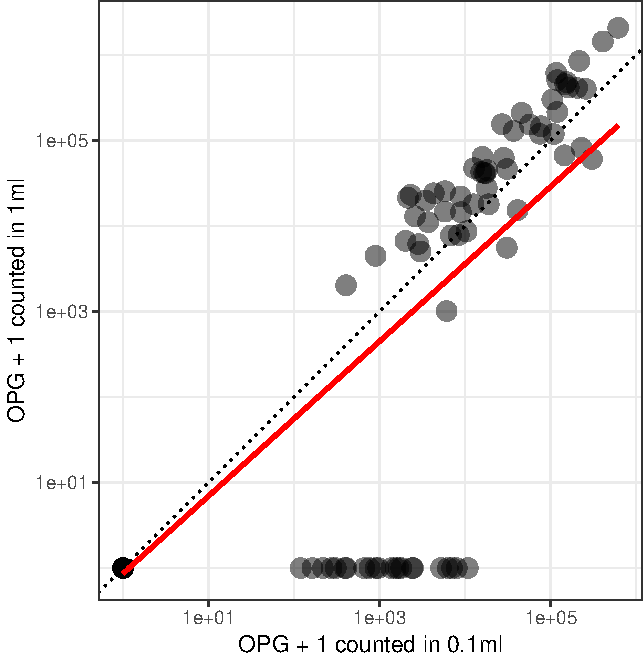
\includegraphics{Data_Analysis_Alice_files/figure-latex/oocystsDetec-1.pdf}

22 new samples were detected while diluting by 0.1mL PBS instead of 1mL
before counting in Neubauer chamber.

Adjusted R-squared = 0.81 represents the amount of variation in y
explained by x.

\subsection{OPG that we keep}\label{opg-that-we-keep}

Number of Mus musculus caught with OPG values: 463

\begin{verbatim}
## `geom_smooth()` using method = 'loess' and formula 'y ~ x'
\end{verbatim}

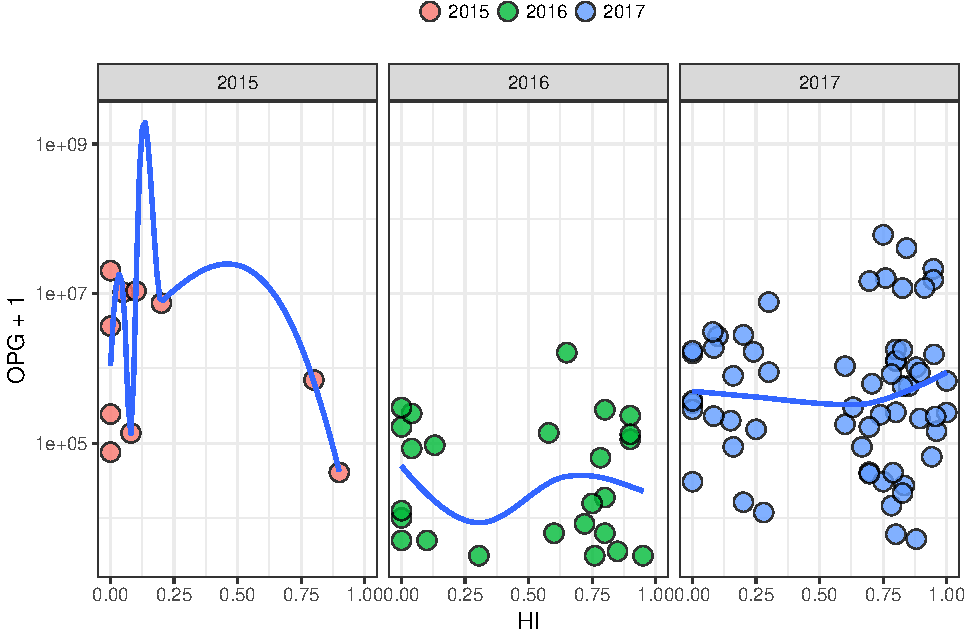
\includegraphics{Data_Analysis_Alice_files/figure-latex/oocystssmooth-1.pdf}

\section{Eimeria detection PCR}\label{eimeria-detection-pcr}

PCR positive = one of the 3 other markers than AP5 sequenced (Ap5 was
used for detection only, the other markers for confirmation)

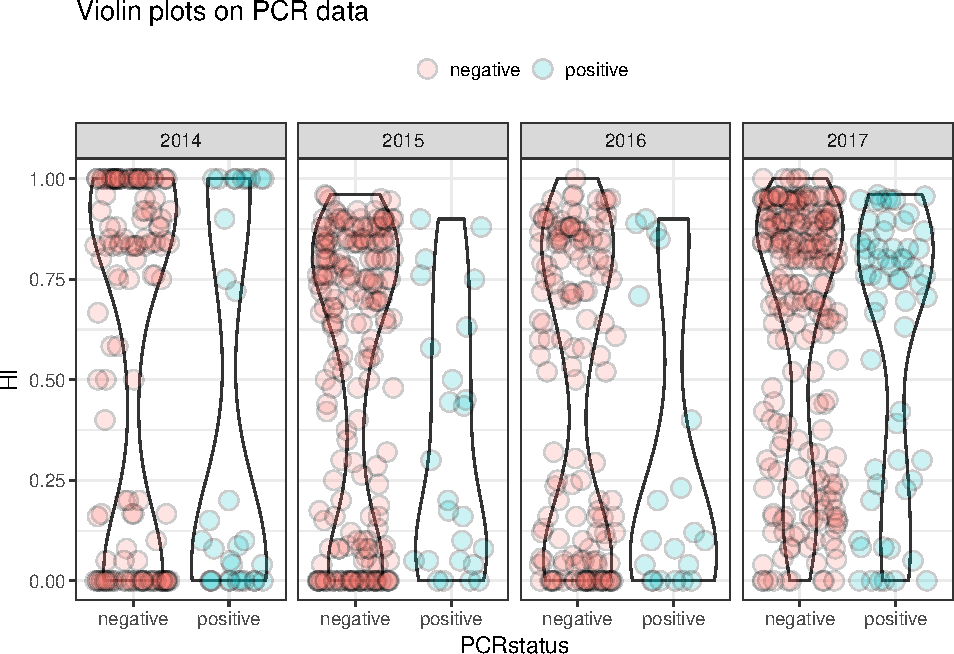
\includegraphics{Data_Analysis_Alice_files/figure-latex/pcr-1.pdf}

PCR positive = one of the 3 markers 18S, COI or ORF470) gave a sequence.
Number of Mus musculus caught with PCR performed: 560

\section{General stats on sampling}\label{general-stats-on-sampling}

\begin{verbatim}
## [1] 577
\end{verbatim}

\begin{verbatim}
## [1] 136
\end{verbatim}

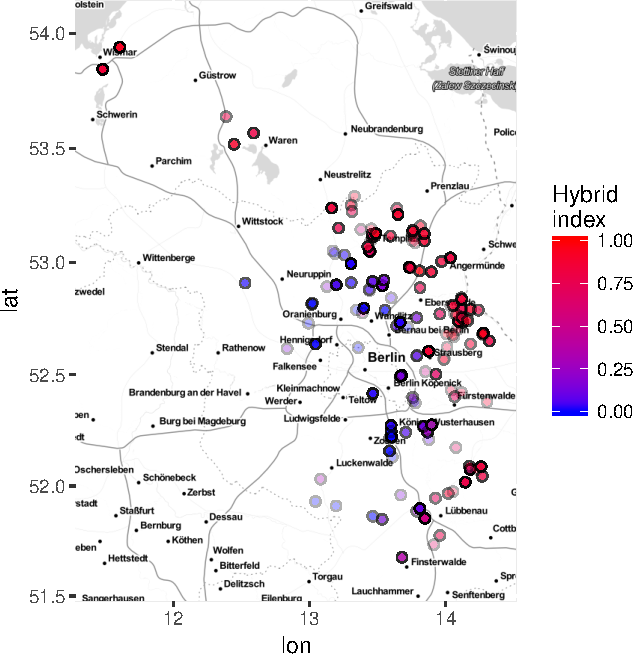
\includegraphics{Data_Analysis_Alice_files/figure-latex/generalstats-1.pdf}

\begin{verbatim}
## [1] 4.222222
\end{verbatim}

\begin{itemize}
\item
  Some information regarding latitude and longitude are missing for the
  following mice:
\item
  We still miss info (HI) on the following mice (ask Jarda):
\end{itemize}

AA\_0411, AA\_0412, AA\_0420, AA\_0464

\section{General informations on
HMHZ}\label{general-informations-on-hmhz}

\begin{itemize}
\item
  577 mice were captured over three years, from 136 farms
\item
  On average, 4.22 mice were caught per farm (95\% CI 0.41)
\item
  \textbf{Hybrid indexes} were calculated as ratio of M.m.d/M.m.m
  alleles (between 4 and 14, on average 13 loci)
\end{itemize}

\begin{figure}
\centering
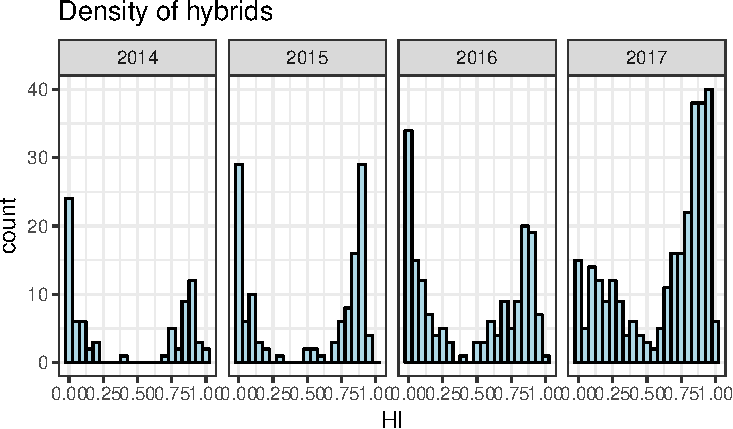
\includegraphics{Data_Analysis_Alice_files/figure-latex/plotDensHI-1.pdf}
\caption{\label{fig:plot1}Number of animals caught along the hybrid
index}
\end{figure}

\section{Prevalence of our 3 different
methods}\label{prevalence-of-our-3-different-methods}

\subsection{Prevalence tables}\label{prevalence-tables}

\begin{longtable}[]{@{}lrrr@{}}
\caption{Prevalence of Eimeria per year, based on oocyst
flotation}\tabularnewline
\toprule
& 2015 & 2016 & 2017\tabularnewline
\midrule
\endfirsthead
\toprule
& 2015 & 2016 & 2017\tabularnewline
\midrule
\endhead
FALSE & 92.0 & 126.00 & 149.00\tabularnewline
TRUE & 10.0 & 25.00 & 61.00\tabularnewline
total & 102.0 & 151.00 & 210.00\tabularnewline
prevalence(\%) & 9.8 & 16.56 & 29.05\tabularnewline
\bottomrule
\end{longtable}

\begin{longtable}[]{@{}lrrr@{}}
\caption{Prevalence of Eimeria per year, based on PCR detection. A mouse
was considered infected by Eimeria if one of the 3 markers (COI, 18S or
ORF470) gave a sequence}\tabularnewline
\toprule
& 2015 & 2016 & 2017\tabularnewline
\midrule
\endfirsthead
\toprule
& 2015 & 2016 & 2017\tabularnewline
\midrule
\endhead
FALSE & 140.00 & 148.00 & 182.00\tabularnewline
TRUE & 12.00 & 19.00 & 59.00\tabularnewline
total & 152.00 & 167.00 & 241.00\tabularnewline
prevalence(\%) & 7.89 & 11.38 & 24.48\tabularnewline
\bottomrule
\end{longtable}

\begin{longtable}[]{@{}lrrr@{}}
\caption{Prevalence of Eimeria per year, based on qPCR in cecum and
ileum}\tabularnewline
\toprule
& 2015 & 2016 & 2017\tabularnewline
\midrule
\endfirsthead
\toprule
& 2015 & 2016 & 2017\tabularnewline
\midrule
\endhead
FALSE & 0 & 134.00 & 160.0\tabularnewline
TRUE & 0 & 31.00 & 39.0\tabularnewline
total & 0 & 165.00 & 199.0\tabularnewline
prevalence(\%) & NaN & 18.79 & 19.6\tabularnewline
\bottomrule
\end{longtable}

\begin{longtable}[]{@{}lrrr@{}}
\caption{Prevalence of Eimeria per year, based on all detections
methods. A mouse was considered infected by Eimeria if one of the 3
markers (COI, 18S or ORF470) gave a sequence, OR if it had a positive
count of oocysts in its feces, OR if it was qPCR positive in cecum
tissue}\tabularnewline
\toprule
& 2015 & 2016 & 2017\tabularnewline
\midrule
\endfirsthead
\toprule
& 2015 & 2016 & 2017\tabularnewline
\midrule
\endhead
negative & 146.00 & 122.00 & 158.00\tabularnewline
positive & 17.00 & 45.00 & 89.00\tabularnewline
total & 163.00 & 167.00 & 247.00\tabularnewline
prevalence(\%) & 10.43 & 26.95 & 36.03\tabularnewline
\bottomrule
\end{longtable}

\subsection{OPG-PCR}\label{opg-pcr}

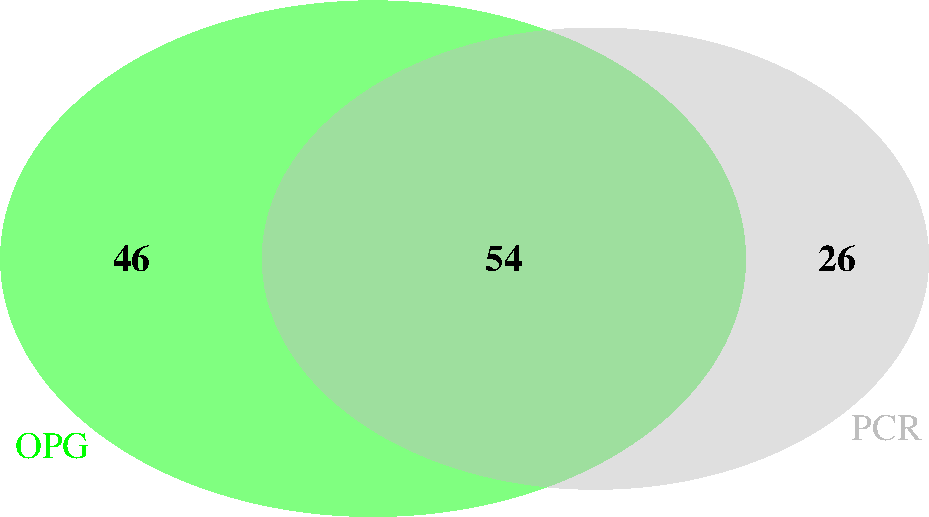
\includegraphics{Data_Analysis_Alice_files/figure-latex/opgpcr-1.pdf}

\begin{verbatim}
## (polygon[GRID.polygon.502], polygon[GRID.polygon.503], polygon[GRID.polygon.504], polygon[GRID.polygon.505], text[GRID.text.506], text[GRID.text.507], text[GRID.text.508], text[GRID.text.509], text[GRID.text.510])
\end{verbatim}

\subsection{OPG-qPCR}\label{opg-qpcr}

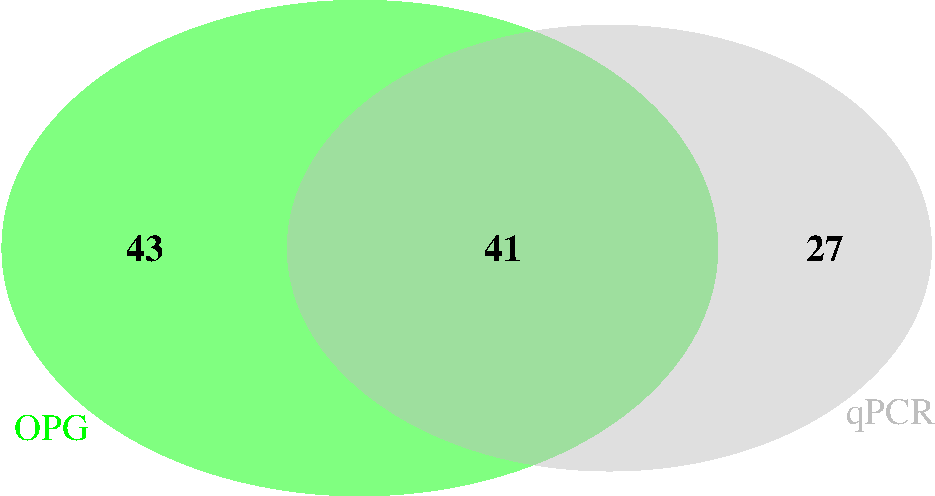
\includegraphics{Data_Analysis_Alice_files/figure-latex/opgpcrVenn-1.pdf}

\begin{verbatim}
## (polygon[GRID.polygon.511], polygon[GRID.polygon.512], polygon[GRID.polygon.513], polygon[GRID.polygon.514], text[GRID.text.515], text[GRID.text.516], text[GRID.text.517], text[GRID.text.518], text[GRID.text.519])
\end{verbatim}

\subsection{OPG-qPCR-PCR}\label{opg-qpcr-pcr}

Discussed with Stuart:

\begin{itemize}
\tightlist
\item
  Test distributions 0 or counts. Test all vs only infected
  (``intensity'') distribution. We should be able to fit the
  distribution of infected on all. Zeros are data. Stochastic move.
\item
  Separation of the zero class. balanced design case/control
  \textasciitilde{} 400 +/-70infectés SNPchip.
\item
  H0: no differences are observed
\item
  Separate \textless{}0.5 and \textgreater{}0.5 to see the species
  effect
\item
  timing : WHEN (for my thesis?)
\end{itemize}


\end{document}
